
\begin{question}
Match ACF and PACF with their corresponding ARMA processes:


\begin{figure}[H]
	\centering
	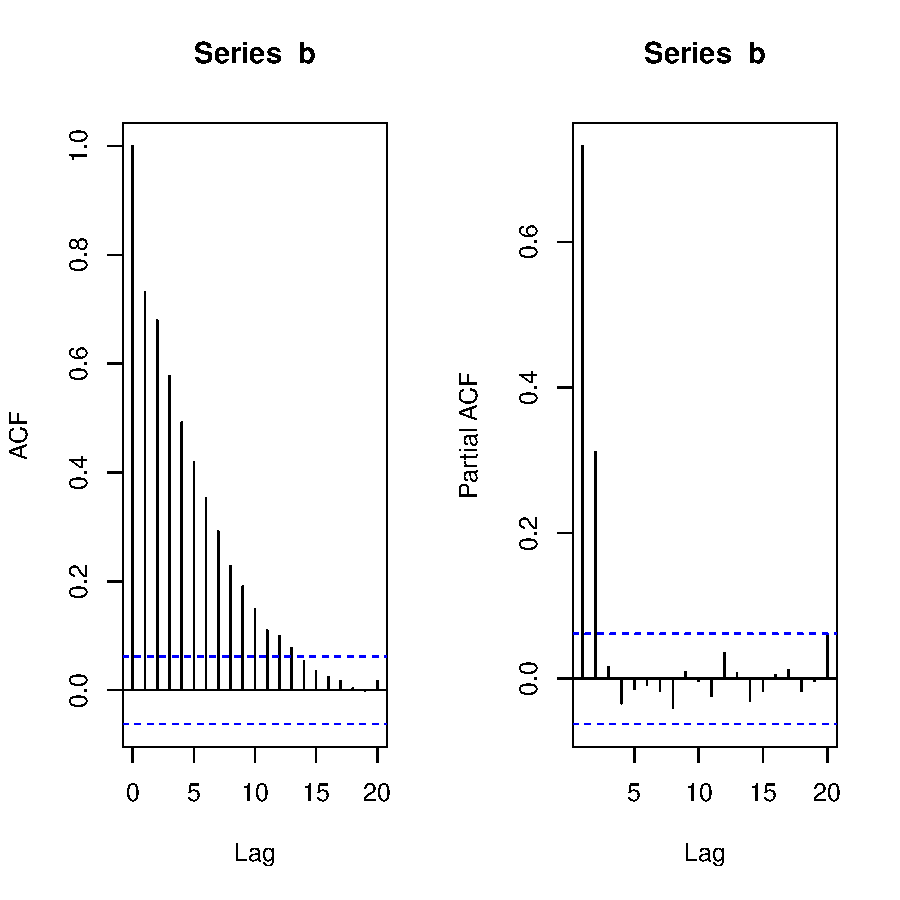
\includegraphics{unnamed-chunk-1-2.pdf}
	\caption{plot of chunk unnamed-chunk-1}
\end{figure}


\begin{figure}[H]
	\centering
	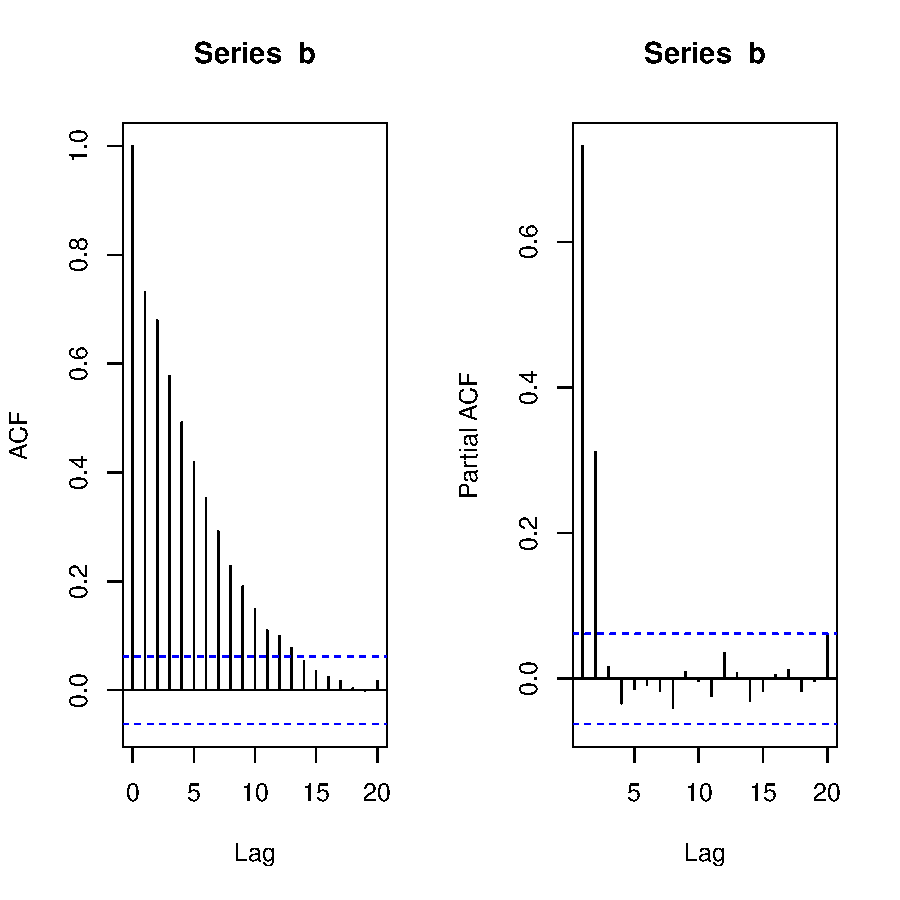
\includegraphics{unnamed-chunk-1-2.pdf}
	\caption{plot of chunk unnamed-chunk-1}
\end{figure}


\begin{figure}[H]
	\centering
	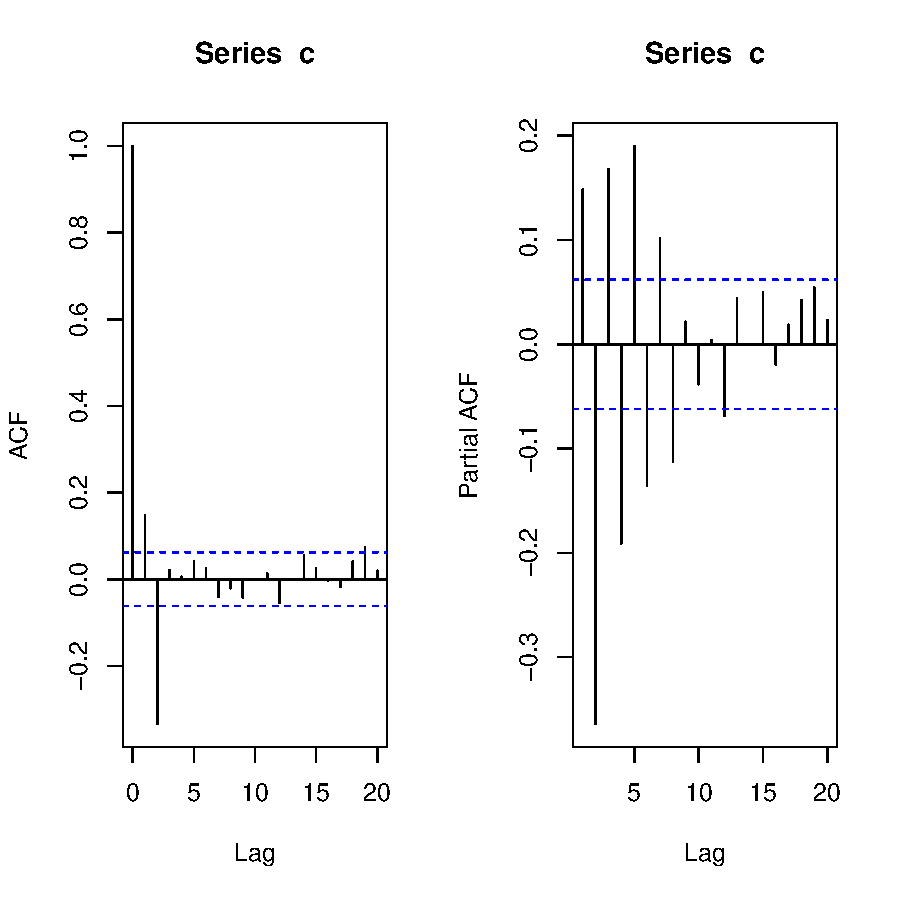
\includegraphics{unnamed-chunk-1-3.pdf}
	\caption{plot of chunk unnamed-chunk-1}
\end{figure}


\begin{figure}[H]
	\centering
	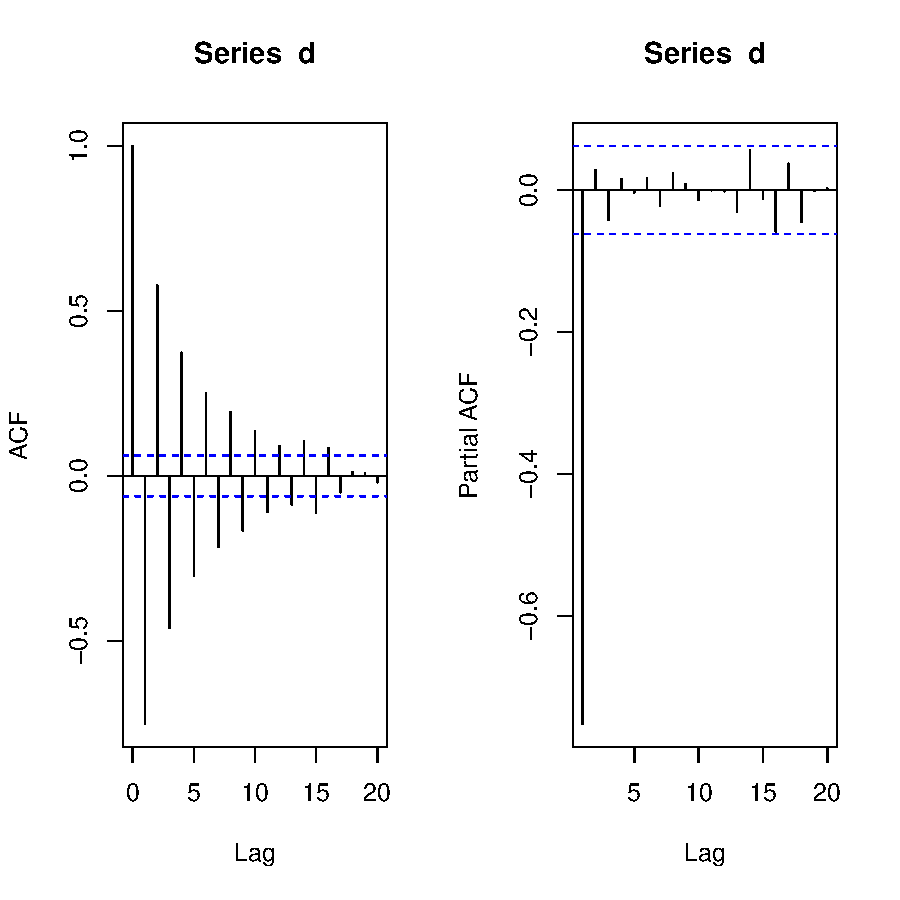
\includegraphics{unnamed-chunk-1-4.pdf}
	\caption{plot of chunk unnamed-chunk-1}
\end{figure}




\begin{enumerate}
\def\labelenumi{\arabic{enumi}.}
\item
  ARMA(2,0)
\item
  ARMA(1,0)
\item
  ARMA(0,2)
\item
  ARMA(2,2)
\end{enumerate}

Write down in the solution the sequence of numbers without spaces or delimeters corresponding to pairs of ACF and PACF in each case (e.g.~4231).
\end{question}

\begin{solution}
A gradual geometrically declining ACF and a PACF that is significant for only a few lags indicate an AR process. MA process shows a gradually geometrically declining PACF and the ACF has a few significant lags. An ARMA process is indicated by geometrically filling ACF and PACF.
\end{solution}

